\documentclass{standalone}
\usepackage{tikz}
\usepackage{ctex,siunitx,ninecolors}
\setCJKmainfont{Noto Serif CJK SC}
\usepackage{tkz-euclide}
\usepackage{amsmath}
\usepackage{wasysym}
\usetikzlibrary{patterns, calc}
\usetikzlibrary{decorations.pathmorphing, decorations.pathreplacing, decorations.shapes,3d}
\begin{document}
\small
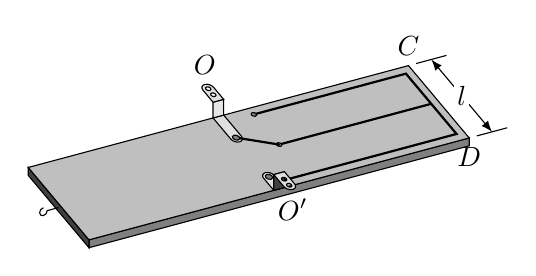
\begin{tikzpicture}[>=latex,z={(15:10mm)},x={(130:10mm)}]
  \begin{scope}[canvas is yz plane at x=-0.6]
    \draw[fill=gray](0,-2.5)rectangle(-0.1,2.5);
  \end{scope}
  \begin{scope}[canvas is xy plane at z=-2.5]
    \draw[fill=darkgray](0.6,-0.1)rectangle(-0.6,0);
  \end{scope}
  \begin{scope}[canvas is yz plane at x=0]
    \draw(-0.05,-2.5)--++(0,-0.15)arc(90:360:0.05);
  \end{scope}
  \begin{scope}[canvas is zx plane at y=0]
    \draw[fill=lightgray](-2.5,-0.6)rectangle(2.5,0.6);
    \draw[thick](0.4,0)--(2.4,0);
    \draw[thick](0.4,0.5)--(2.4,0.5)--(2.4,-0.5)--(0,-0.5);
    \draw[fill=gray](0.4,0.5)circle(0.03)(0.4,0)circle(0.03);
    \draw[fill=lightgray!50](-0.07,-0.6)--(-0.07,-0.4)arc(180:0:0.07)--(0.07,-0.6)--cycle;
    \draw[fill=lightgray!50](-0.07,0.6)--(-0.07,0.25)arc(180:360:0.07)--(0.07,0.6)--cycle;
    \draw[thick,line cap=round](0,0.25)--(0.4,0);
    \draw[fill=gray](0,0.25)circle(0.04);
    \draw[fill=gray](0,-0.4)circle(0.04);
    \draw [thin] (2.6,0.6)--(3.0,0.6)(2.6,-0.6)--(3.0,-0.6);
    \draw[thin,<->](2.8,-0.6)--(2.8,0.6)node[midway,fill=white,inner sep=1pt]{$l$};
    \node at (2.5,0.6)[above]{$C$};
    \node at (2.5,-0.6)[below]{$D$};
  \end{scope}
  \begin{scope}[canvas is yz plane at x=-0.6]
    \draw[fill=darkgray](0,-0.07)rectangle(0.2,0.07);
  \end{scope}
  \begin{scope}[canvas is yz plane at x=0.6]
    \draw[fill=lightgray!40](0,-0.07)rectangle(0.2,0.07);
  \end{scope}
  \begin{scope}[canvas is zx plane at y=0.2]
    \draw[fill=lightgray!50,even odd rule](-0.07,-0.6)--(-0.07,-0.8)arc(180:360:0.07)--(0.07,-0.6)--cycle(0,-0.7)circle(0.03)(0,-0.8)circle(0.03);
    \draw[fill=lightgray!50,even odd rule](-0.07,0.6)--(-0.07,0.8)arc(180:0:0.07)--(0.07,0.6)--cycle(0,0.7)circle(0.03)(0,0.8)circle(0.03);
    \node at (0,0.87)[above]{$O$};
    \node at (0,-0.87)[below]{$O'$};
  \end{scope}
\end{tikzpicture}
\end{document}